\section{Battery State of Charge}
TODO:
\begin{itemize}
	\item find variable for power and substitute
	\item make arrows for delta give space between arrow tip and box
	\item begin more thorough pass through on text and explaining where things go
\end{itemize}
BEBs must also maintain their state of charge above a minimum threshold. Let $h_{ij+1}$ be the state of charge for bus $i$ at the beginning of stop $j$. Each bus has an initial state of charge defined by $h_{i0}$ as shown in figure \ref{fig:hPlacement}. 
\begin{figure*}
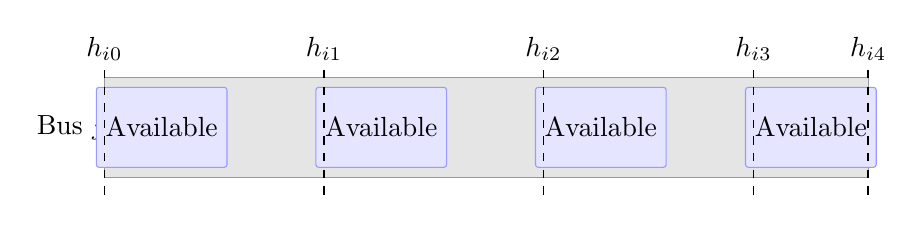
\begin{tikzpicture}
\node[rectangle, draw=black!40, fill=black!10, minimum width=0.8\textwidth, minimum height=0.5in](charger1Box) at (0.5\textwidth,1){};
	\node(bus1BoxLabel) at (0.065\textwidth, 1){Bus $j$}; 
	\node[rectangle, draw=blue!40, fill=blue!10, minimum width=0.12\textwidth, minimum height=0.4in, rounded corners=1pt] at (0.16\textwidth,1){Available};
	\node[rectangle, draw=blue!40, fill=blue!10, minimum width=0.12\textwidth, minimum height=0.4in, rounded corners=1pt] at (0.39\textwidth,1){Available};
	\node[rectangle, draw=blue!40, fill=blue!10, minimum width=0.12\textwidth, minimum height=0.4in, rounded corners=1pt] at (0.62\textwidth,1){Available};
	\node[rectangle, draw=blue!40, fill=blue!10, minimum width=0.12\textwidth, minimum height=0.4in, rounded corners=1pt] at (0.84\textwidth,1){Available};

	\node(h0High) at (0.1\textwidth,2){$h_{i0}$};
	\node(h0Low) at (0.1\textwidth,0.05){};
	\draw[dashed, line width=0.5pt] (h0High) -- (h0Low.center);

	\node(h1High) at (0.33\textwidth,2){$h_{i1}$};
	\node(h1Low) at (0.33\textwidth,0.05){};
	\draw[dashed, line width=0.5pt] (h1High) -- (h1Low.center);

	\node(h0High) at (0.56\textwidth,2){$h_{i2}$};
	\node(h0Low) at (0.56\textwidth,0.05){};
	\draw[dashed, line width=0.5pt] (h0High) -- (h0Low.center);

	\node(h0High) at (0.78\textwidth,2){$h_{i3}$};
	\node(h0Low) at (0.78\textwidth,0.05){};
	\draw[dashed, line width=0.5pt] (h0High) -- (h0Low.center);

	\node(h0High) at (0.9\textwidth,2){$h_{i4}$};
	\node(h0Low) at (0.9\textwidth,0.05){};
	\draw[dashed, line width=0.5pt] (h0High) -- (h0Low.center);
\end{tikzpicture}
\caption{State of Charge Variables}
\label{fig:hPlacement}
\end{figure*}

This can be constrained as
\begin{equation}
	d_{i0} = \text{initialSoc}_{i} \ \forall i.
\end{equation}
\begin{figure*}
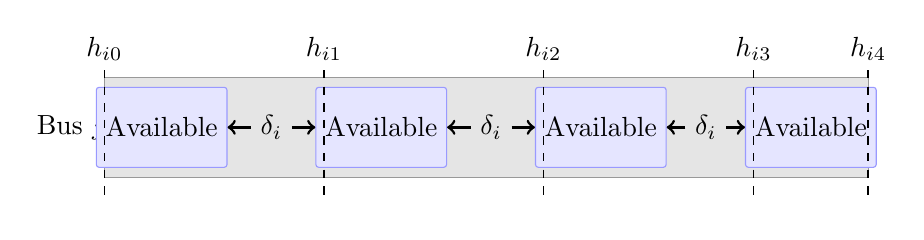
\begin{tikzpicture}
\node[rectangle, draw=black!40, fill=black!10, minimum width=0.8\textwidth, minimum height=0.5in](charger1Box) at (0.5\textwidth,1){};
	\node(bus1BoxLabel) at (0.065\textwidth, 1){Bus $j$}; 
	\node[rectangle, draw=blue!40, fill=blue!10, minimum width=0.12\textwidth, minimum height=0.4in, rounded corners=1pt](avail1) at (0.16\textwidth,1){Available};
	\node[rectangle, draw=blue!40, fill=blue!10, minimum width=0.12\textwidth, minimum height=0.4in, rounded corners=1pt](avail2) at (0.39\textwidth,1){Available};
	\node[rectangle, draw=blue!40, fill=blue!10, minimum width=0.12\textwidth, minimum height=0.4in, rounded corners=1pt](avail3) at (0.62\textwidth,1){Available};
	\node[rectangle, draw=blue!40, fill=blue!10, minimum width=0.12\textwidth, minimum height=0.4in, rounded corners=1pt](avail4) at (0.84\textwidth,1){Available};

	\node(h0High) at (0.1\textwidth,2){$h_{i0}$};
	\node(h0Low) at (0.1\textwidth,0.05){};
	\draw[dashed, line width=0.5pt] (h0High) -- (h0Low.center);

	\node(h1High) at (0.33\textwidth,2){$h_{i1}$};
	\node(h1Low) at (0.33\textwidth,0.05){};
	\draw[dashed, line width=0.5pt] (h1High) -- (h1Low.center);

	\node(h0High) at (0.56\textwidth,2){$h_{i2}$};
	\node(h0Low) at (0.56\textwidth,0.05){};
	\draw[dashed, line width=0.5pt] (h0High) -- (h0Low.center);

	\node(h0High) at (0.78\textwidth,2){$h_{i3}$};
	\node(h0Low) at (0.78\textwidth,0.05){};
	\draw[dashed, line width=0.5pt] (h0High) -- (h0Low.center);

	\node(h0High) at (0.9\textwidth,2){$h_{i4}$};
	\node(h0Low) at (0.9\textwidth,0.05){};
	\draw[dashed, line width=0.5pt] (h0High) -- (h0Low.center);

	\node(delta1) at (0.275\textwidth,1){$\delta_i$};
	\draw[->, line width=1pt] (delta1.west) -- (avail1.east);
	\draw[->, line width=1pt] (delta1.east) -- (avail2.west);
	\node(delta2) at (0.505\textwidth,1){$\delta_i$}; 
	\draw[->, line width=1pt] (delta2.west) -- (avail2.east);
	\draw[->, line width=1pt] (delta2.east) -- (avail3.west);
	\node(delta3) at (0.73\textwidth,1){$\delta_i$}; 
	\draw[->, line width=1pt] (delta3.west) -- (avail3.east);
	\draw[->, line width=1pt] (delta3.east) -- (avail4.west);
\end{tikzpicture}
\caption{Placement for $\delta_i$}
\label{fig:hPlacement}
\end{figure*}

The transition from one start to the next is computed as
\begin{equation}
	h_{ij} = h_{ij-1} - \delta_i + \left(\sum_k\sigma_{ijk}\right )\text{power}\cdot(d_{ij} - a_{ij}) 
\end{equation}
but because this introduces a bilinear term, we can alternatively express this constraint as
\begin{equation} \begin{aligned}
	h_{ij} & \le h_{ij-1} - \delta_i + \text{power}\cdot(d_{ij} - a_{ij}) - M(1 - \sum_k\sigma_{ijk})\\
	h_{ij} & \ge h_{ij-1} - \delta_i + \text{power}\cdot(d_{ij} - a_{ij}) + M(1 - \sum_k\sigma_{ijk})\\
	h_{ij} & \le h_{ij-1} - \delta_i - M\sum_k\sigma_{ijk}\\
	h_{ij} & \ge h_{ij-1} - \delta_i + M\sum_k\sigma_{ijk}\\
\end{aligned} \end{equation}
Which can be expressed in standard form as
\begin{equation} \begin{aligned}
	h_{ij} - h_{ij-1} - \text{power}\cdot d_{ij} + \text{power}\cdot a_{ij} - M\sum_k\sigma_{ijk} &\le -\left(\delta_i + M\right) \\
	-h_{ij} + h_{ij-1} + \text{power}\cdot d_{ij} - \text{power}\cdot a_{ij} - M\sum_k\sigma_{ijk} &\le \delta_i - M \\
	h_{ij} - h_{ij-1} + M\sum_k\sigma_{ijk} &\le -\delta_i \\
	-h_{ij} + h_{ij-1} + M\sum_k\sigma_{ijk} & \le \delta_i \\
\end{aligned} \end{equation}
and finally,
\begin{equation} \begin{aligned}
	\begin{bmatrix}1  & -1 & -\text{power} & \text{power}   & -M_k \\
		       -1 & 1  & \text{power}  & -\text{power}  & -M_k \\
		       1  & -1 & 0             & 0              & M_k  \\
		       -1 & 1  & 0             & 0              & M_k  \\
	\end{bmatrix}
	\begin{bmatrix}h_{ij} \\ h_{ij-1} \\ d_{ij} \\ a_{ij} \\ \sigma_{ijk} \end{bmatrix} \le 
		\begin{bmatrix}-\delta_i - M \\ \delta_i - M \\ -\delta_i \\ \delta_i \end{bmatrix}
\end{aligned} \end{equation}
If the bus end the day in the station (as is common), there is one final state of charge value that is computed as above without a route discharge parameter as
\begin{equation}
\begin{bmatrix}1  & -1 & -\text{power} & \text{power}   & -M_k \\
		       -1 & 1  & \text{power}  & -\text{power}  & -M_k \\
		       1  & -1 & 0             & 0              & M_k  \\
		       -1 & 1  & 0             & 0              & M_k  \\
	\end{bmatrix}
	\begin{bmatrix}h_{ij} \\ h_{ij-1} \\ d_{ij} \\ a_{ij} \\ \sigma_{ijk} \end{bmatrix} \le 
		\begin{bmatrix}- M \\ - M \\ 0 \\ 0 \end{bmatrix}.
\end{equation}
Now that the state of charge is defined, the final constraint ensures that the minimum battery state of charge is kept above some minimum threshold, denoted $h_{\text{min}}$. These constraints are given as
\begin{equation}
	-h_{ij} \le -h_{\text{min}} \ \forall i,j
\end{equation}
or 
\begin{equation} \begin{aligned}
	\begin{bmatrix}0 & \hdots & 0 & 1_{h} & 0 & \hdots & 0\end{bmatrix} \mathbf{y} &\le \mathbf{1}\cdot h_{\text{min}}\\ 
		H\mathbf{y} &\le \mathbf{b}_h
\end{aligned} \end{equation}

